\chapter{Результаты и их обсуждение}
\label{ch:results}

\section{Экспериментальная установка}

%в установке есть ключевые вещи: углекислый газ при некоторых давлениях, дросселировался, был термометр для определения разности температур, было то-то то-то и всё это находилось в термостате. полное описание установки находится в приложении. просто, что контроллировалось, а как контроллировалось - это вторичный вопрос.

Схема установки для исследования эффекта Джоуля–Томсона в углекислом газе представлена на рис. 2. Углекислый газ дросселировался через трубку с пористой перегородкой. Температура газа до входа в трубку задавалась при помощи термостата. Температура газа при выходе из трубки измерялась термометром. Трубка была сделана из материала с малой теплопроводностью, чтобы считать процесс дросселирования адиабатическим.

\begin{figure}[h!]
        \centering
        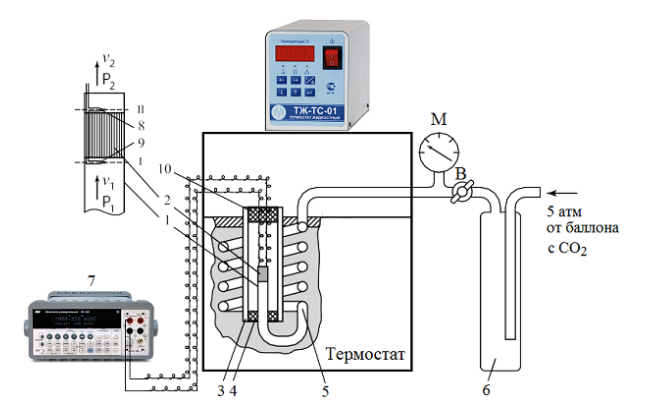
\includegraphics[scale=1]{img/ustj.jpg}
\end{figure} 
\begin{center}
    Рис. 2. Углекислый газ дросселировался через трубку с пористой перегородкой. Температура газа до входа в трубку задавалась при помощи термостата. Температура газа при выходе из трубки измерялась термометром. Трубка была сделана из материала с малой теплопроводностью, чтобы считать процесс дросселирования адиабатическим.
\end{center}

\section{Обработка результатов измерений}

Для того, чтобы определить коэффициенты Джоуля-Томсона для для начальных температур: 20 \celsius, 30 \celsius, 40 \celsius, 50 \celsius, экспериментально нашли зависимость $\Delta T (\Delta P)$ для соответствующих начальных температур ( результаты см. в Приложении Б.). Чтобы по зависимости $\Delta T (\Delta P)$ определить коэффициенты Джоуля-Томсона, построили график зависимости $\Delta T (\Delta P)$ (см. рис. 2). Из графика видно, что зависимость $\Delta T (\Delta P)$ линейная, что соответствует ожиданиям, которые следовали из определения коэффициента Джоуля-Томсона. По угловым коэффициентам наклона графиков нашли коэффициенты Джоуля-Томсона для каждой из начальных температур.

\begin{figure}[ht]
\centering
    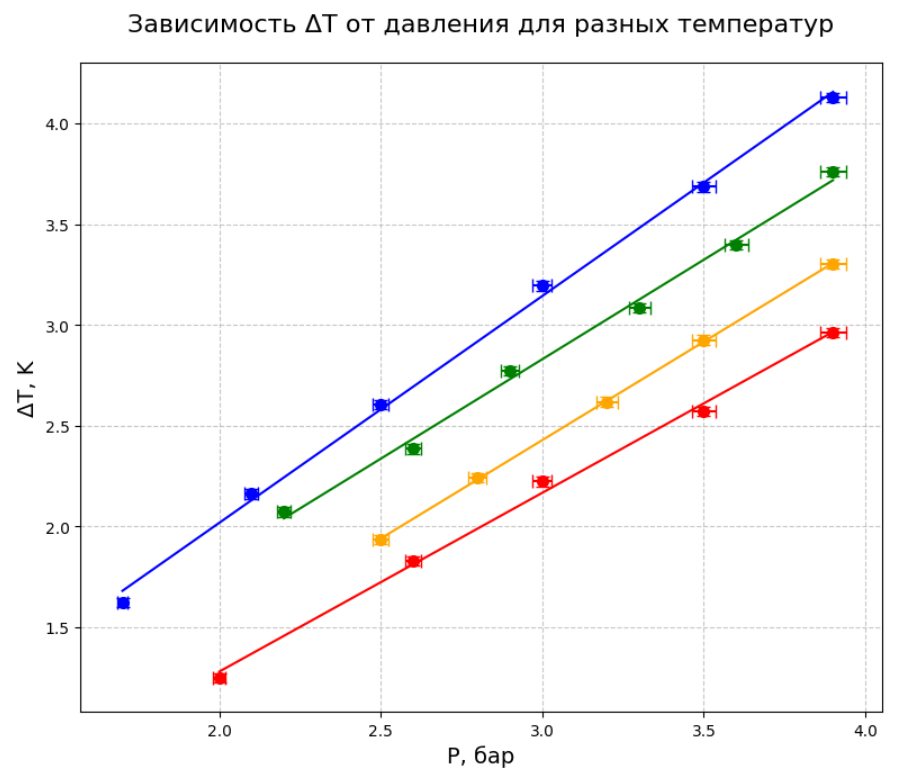
\includegraphics[width = 0.8\textwidth]{img/dT(dP).png}
    \begin{center}
    Рис. 2. График зависимости $\Delta T (\Delta P)$. На графике синие точки - это данные, полученные для температуры термостата 20 \celsius, зелёные - 30 \celsius, жёлтые - 40 \celsius, красные - 50 \celsius. Линиями соответствующих цветов проведены линии аппроксимации, по коэффициенту наклона которых определялись коэффициенты Джоуля-Томсона для разных температур. %(полностью описание) для чего, что на рисунке
    \end{center}
\end{figure}

\begin{table}[h]
\centering
\begin{tabular}{|c|c|}
\hline
$t_0$, °C & $\mu$, K/бар \\ \hline
$20.00$ & $1.13 \pm 0.01$  \\ \hline
$30.00$ & $0.99 \pm 0.02$  \\ \hline
$40.00$ & $0.98 \pm 0.02$  \\ \hline
$50.00$ & $0.89 \pm 0.02$  \\ \hline
\end{tabular}
\caption{Коэффициенты Джоуля-Томсона для начальных температур: 20 \celsius, 30 \celsius, 40 \celsius, 50 \celsius}
\end{table}

\begin{figure}[ht]
\centering
    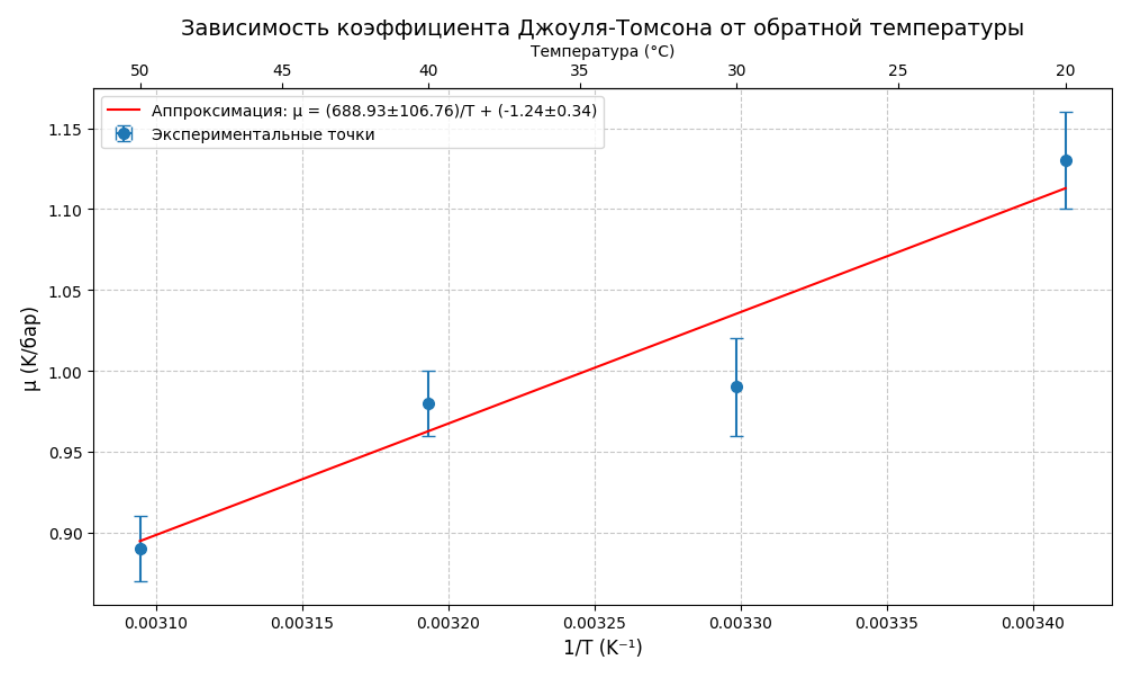
\includegraphics[width = \textwidth]{img/u(1T).png}
    \begin{center}
    Рис. 3. График зависимости $\mu (1/T)$. На графике синие точки - это данные, полученные для каждой температуры термостата: 20 \celsius, 30 \celsius, 40 \celsius, 50 \celsius. Красная линия проведена, чтбы показать, как аппроксимируется зависимость  $\mu (1/T)$.  %(полностью описание) для чего, что на рисунке
    \end{center}
\end{figure}

Для того, чтобы найти поправки a и b из уравнения Ван-Дер-Ваальса для углекислого газа, построили график зависимости коэффициента Джоуля-Томсона $\mu$ от обратной температуры $1/T$ (см. рис. 3). %Да, я помню, что лучше строить 1000/T

Параметры графика, которые входят в выражение для нахождения поправок a и b,  получились следующими:
\[k = (0.7 \pm 0.1) \cdot 10^3 \ \frac{K^2}{\text{бар}} \ \ \ \ \ \ \ \mu_0 = (-1.2 \pm 0.3) \ \frac{K}{\text{бар}}, \] где k - коэффициент наклона графика, $\mu_0$ - значение при 1/T стремящемся к нулю.

Используя эти параметры нашли искомые поправки $a$ и $b$ по формулам:
\[a = \frac{kRC_p}{2} \hspace{30pt}  b= \mu_0 C_p,\] где $C_p = 37,1 \frac{\text{Дж}}{\text{моль} \cdot \text{К}}$ табличное значение \cite{Lab}.

\[a  = (1,48 \pm 0,24) \  \frac{H\cdot\text{ м} ^4}{\text{моль} ^2}  \ \ \ \ \ \ \ b = (0.81 \pm 0.19) \cdot 10^{-3} \frac{\text{м} ^3}{\text{моль}}\]

Полученные значения a и b разошлись с табличными $a_{\text{табл}} = 0.365$ $\frac{\text{Н·м}^4}{\text{моль}^2}$, $b_{\text{табл}} = 4.28 \cdot 10^{-3}$ $\frac{\text{м}^3}{\text{моль}}$ \cite{Lab}.

Для понимания того, как происходит изменение температуры газа при дросселировании также полезно знать температуру инверсии $T_{\text{инв}}$, которая определяется, как $T_{\text{инв}} = \frac{2a}{Rb}$. Для углекислого газа получили $T_{\text{инв}} = (0.44 \pm 0.12) \cdot 10^3 \ K$. Полученное значение отличается от табличного $T_{{{\text{инв}}}_{\text{табл}}} = 2 \cdot 10^{3} K$ \cite{Lab}. 

Расхождение полученных значений a, b и $T_\text{инв}$ с табличными говорит о том, что модель газа Ван-дер-Ваальса не позволяет описать поведение углекислого газа.

%значащие цифры погрешности
